\documentclass[handout]{beamer}

\usepackage[utf8]{inputenc} % Language and font encoding
\usepackage[icelandic]{babel}
\usepackage[T1]{fontenc}


\usepackage{tikz}
\usepackage[listings,theorems]{tcolorbox}
\usepackage{booktabs}
\usepackage{minted} %Minted and configuration
\usemintedstyle{default}

\renewcommand{\theFancyVerbLine}{\sffamily \arabic{FancyVerbLine}}
%%%%%%%%%%%
% More math
%%%%%%%%%%%
\newcommand{\Mod}[1]{\ \text{mod}\ #1}

%%%%%%%%%%%%%%%%%%%%%%
% Beamer configuration
%%%%%%%%%%%%%%%%%%%%%%
\setbeamertemplate{navigation symbols}{}
\usecolortheme{dove}
\setbeamercolor{frametitle}{fg=white}

\usebackgroundtemplate%
{%
\vbox to \paperheight{

\includegraphics[width=\paperwidth]{Pics/hi-slide-head-2016}

\vfill
\hspace{0.5cm}
\includegraphics[width=0.3\paperwidth]{Pics/hi-von-logo}
\vspace{0.4cm}
    }%
}

\AtBeginSection[]
{
  \begin{frame}<beamer>
    \frametitle{Yfirlit}
    \tableofcontents[currentsection]
  \end{frame}
}

\setbeamerfont{frametitle}{size=\normalsize}
\addtobeamertemplate{frametitle}{}{\vspace*{0.5cm}}

%%%%%%%%%%%%%%%%%%%%%%%%%
% tcolorbox configuration
%%%%%%%%%%%%%%%%%%%%%%%%%

% Setup from: http://tex.stackexchange.com/a/43329/21638
\tcbset{%
    noparskip,
    colback=gray!10, %background color of the box
    colframe=gray!40, %color of frame and title background
    coltext=black, %color of body text
    coltitle=black, %color of title text 
    fonttitle=\bfseries,
    alerted/.style={coltitle=red, colframe=gray!40},
    example/.style={coltitle=black, colframe=green!20, colback=green!5},
}


%%%%%%%%%%%%%%%%%%%%%%%
% Further configuration
%%%%%%%%%%%%%%%%%%%%%%%
\hypersetup{colorlinks=true,pdfauthor={Eirikur Ernir Thorsteinsson},linkcolor=blue,urlcolor=blue}
\graphicspath{{./Pics/}}

\author{Eiríkur Ernir Þorsteinsson}
\institute{Háskóli Íslands}
\date{Haust 2016}

\title{Stærðfræðimynstur í tölvunarfræði}
\subtitle{Vika 1, seinni fyrirlestur}

\begin{document}

\begin{frame}
\titlepage
\end{frame}

\section{Inngangur}

\begin{frame}{Í síðasta tíma}
\begin{itemize}
 \item Kynntumst hugtakinu um \emph{yrðingar}
 \begin{itemize}
  \item Yrðingar eru fullyrðingar sem eru áreiðanlega sannar eða áreiðanlega ósannar
  \item Yrðingar má tákna með rökbreytum
 \end{itemize}
 \item Sáum rökvirkja sem vinna á yrðingum, sanntöflur, skilgreiningu á jafngildi yrðinga
\end{itemize}
\end{frame}

\section{Hagnýting yrðinga}

\subsection{Forritun}

\begin{frame}[fragile]{Í forritun}
\begin{columns}
\column{0.4\textwidth}
\begin{itemize}
 \item Ýmis form yrðinga koma fyrir í öllum forritunarmálum (sem kennari hefur séð)
 \item Fáið að sjá á næstu vikum í Tölvunarfræði 1 og Tölvunarfræði 1a!
\end{itemize}
\column{0.6\textwidth}
\begin{minted}[fontsize=\scriptsize, frame=lines, label=Yrðingar í Java]{java}
public static void main(String []args) {
  Boolean p = true;
  Boolean q = false;
  // p && q þýðir ``p og q''
  System.out.println(p && q);
  // p && q þýðir ``p eða q''
  System.out.println(p || q);
}
\end{minted}

\end{columns}
\end{frame}

\subsection{Gátur}

\begin{frame}{Lausnir á gátum}
\begin{itemize}
 \item Ýmsar gátur má leysa með því að setja þær fram á yrðingaformi
 \item Brjótum setningar gátunnar niður í yrðingar
 \item Könnum sanngildi yrðinganna
\end{itemize}
\end{frame}

\begin{frame}{Riddarar og ribbaldar}
\pause
\begin{itemize}
 \item Við erum stödd á eyju þar sem íbúar eru annaðhvort riddarar eða ribbaldar
 \begin{itemize}
  \item Riddarar segja alltaf satt
  \item Ribbaldar segja alltaf ósatt
 \end{itemize}
 \item Hittum tvo einstaklinga, $A$ og $B$. 
 \begin{itemize}
  \item $A$ segir: ``$B$ er riddari.''
  \item $B$ segir: ``Við erum af mismunandi gerðum.''
 \end{itemize}
 \item Af hvaða gerðum eru $A$ og $B$?
\end{itemize}
\end{frame}

\begin{frame}{Riddarar og ribbaldar á yrðingaformi}
\begin{itemize}
 \item Látum $p$ vera yrðinguna ``$A$ er riddari''
 \item Látum $p$ vera yrðinguna ``$B$ er riddari''
 \item Hvað getum við fullyrt út frá því sem $A$ sagði? \pause
 \begin{itemize}
  \item Ef $p$ er satt, þá er $q$ satt
  \item Ef $q$ er ósatt, þá er $p$ ósatt
 \end{itemize}
 \item Hvað getum við fullyrt út frá því sem $B$ sagði? \pause
 \begin{itemize}
  \item Ef $p \oplus q$ er satt, þá er $q$ satt
  \item Ef $p \oplus q$ er ósatt, þá er $q$ ósatt
 \end{itemize}
 \item Hvert er sanngildi $(p \leftrightarrow q) \land ((p \oplus q) \leftrightarrow q)$?
\end{itemize}
\end{frame}

\begin{frame}{Riddarar og ribbaldar - sanntafla}
Komumst að sanngildi $(p \leftrightarrow q) \land ((p \oplus q) \leftrightarrow q)$ með sanntöflu:
\begin{center}
\begin{tabular}{ccccc}
\toprule
$p$&$q$&$p \leftrightarrow q$&$p \oplus q$& $(p \oplus q) \leftrightarrow q$\\
\midrule
0&0&1&0&1\\
1&0&0&1&0\\
0&1&0&1&1\\
1&1&1&0&0\\
\bottomrule
\end{tabular}
\end{center}\pause
Fullyrðingarnar standast einungis þegar bæði $A$ og $B$ eru ribbaldar.
\end{frame}

\subsection{Rökrásir}

\begin{frame}{Rökrásir}
\begin{itemize}
 \item Stafrænar rásir eru byggðar upp eins og yrðingar
 \item Notum sanngildin $0$ og $1$ sem ``merki''
 \item Búum til rafrás sem tekur við merkjum $p_1, p_2, \ldots, p_n$ og skilar merkjum $s_1, s_2, \ldots s_n$
 
 \item Notum rökhlið (e. \emph{logic gates}) til að breyta merkjunum
\end{itemize}
\end{frame}

\begin{frame}{Rökrásir}
Getum við búið til rökrás sem táknar yrðinguna $(p \land \lnot q) \lor \lnot r$ með því að nota þessi grunnhlið?
\begin{center}
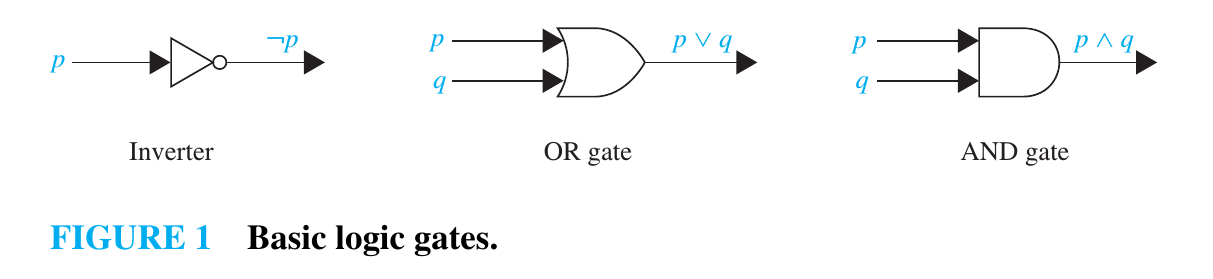
\includegraphics[width=0.8\textwidth]{logic-circuit}\\
\pause
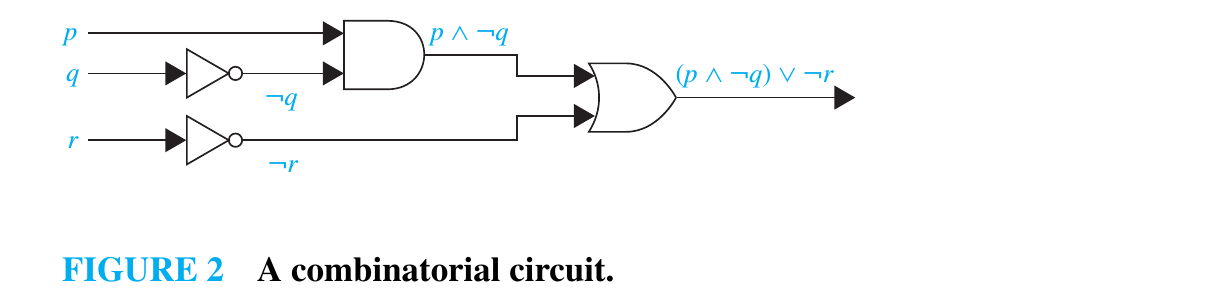
\includegraphics[width=0.8\textwidth]{comi-circuit}
\end{center}
Mynd úr kafla 1.2 í bók
\end{frame}

\section{Jafngildi yrðinga}

\begin{frame}{Jafngildi}
Í síðasta tíma sáum við skilgreiningu á jafngildi:

\begin{tcolorbox}[title=Jafngildi]
Yrðingarnar $p$ og $q$ eru jafngildar (e. \emph{equivalent}) sé $p \leftrightarrow q$ sísanna.
\end{tcolorbox}

Við munum tákna jafngildi með $\equiv$.
\end{frame}

\begin{frame}{De Morgan jafngildin}
Mikilvæg jafngildi sem oft koma upp eru jafngildi/reglur De Morgans, sem eru eftirfarandi:

\[
 \lnot ( p \land q ) \equiv \lnot p \lor \lnot q
\]

\[
 \lnot (p \lor q ) \equiv \lnot p \land \lnot q
\]

\end{frame}

\begin{frame}{De Morgan og sanntöflur}
Sýnum fram á að $\lnot (p \lor q ) \equiv \lnot p \land \lnot q$ með sanntöflu:
\begin{center}
\begin{tabular}{ccccccc}
\toprule
$p$&$q$&$p \lor q$&$\lnot(p \lor q)$&$\lnot p$&$\lnot q$&$\lnot p \land \lnot q$\\
\midrule
0&0&0&1&1&1&1\\
1&0&1&0&0&1&0\\
0&1&1&0&1&0&0\\
1&1&1&0&0&0&0\\
\bottomrule
\end{tabular}
\end{center}
$\lnot (p \lor q ) \leftrightarrow \lnot p \land \lnot q$ er sísanna, svo reglan gildir.
\end{frame}

\begin{frame}{Ýmis jafngildi}
\begin{columns}
\column{0.25\textwidth}
Tafla úr kafla 1.3
\column{0.75\textwidth}
\begin{center}
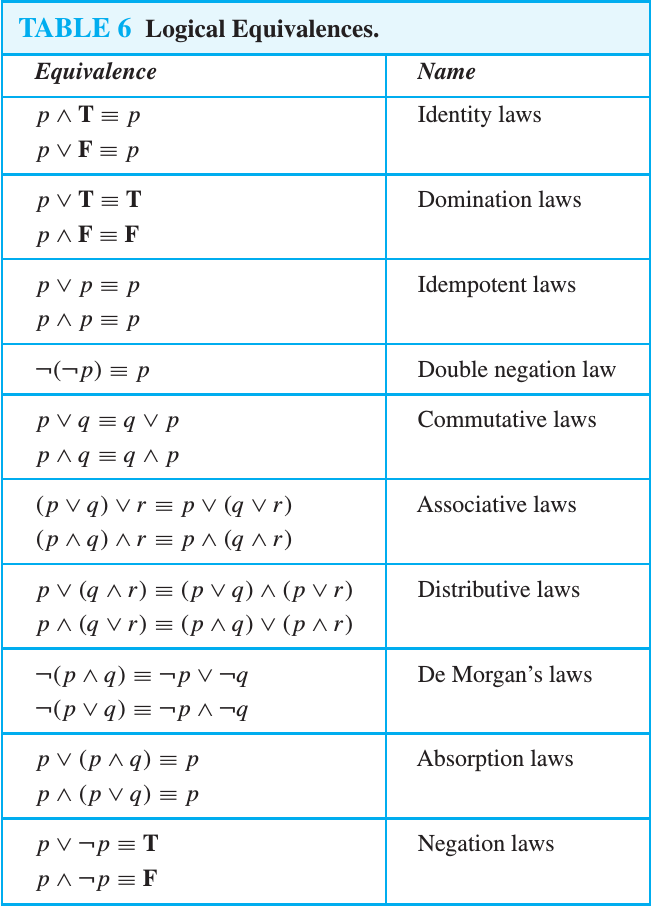
\includegraphics[height=0.8\textheight]{equivalences}
\end{center}
\end{columns}
\end{frame}

\begin{frame}{Sýnt fram á jafngildi}
Við þurfum ekki að nota sanntöflur til að sýna fram á jafngildi. Einföldum ljóta yrðingu:
\begin{align*}
\lnot (p \lor (\lnot p \land q)) &\equiv \lnot p \land \lnot ( \lnot p \land q)\\
&\equiv \lnot p \land (\lnot (\lnot p) \lor \lnot q)\\
&\equiv \lnot p \land (p \lor \lnot q)\\
&\equiv (\lnot p \land p ) \lor (\lnot p \land \lnot q)\\
&\equiv 0 \lor (\lnot p \land \lnot q)\\
&\equiv \lnot p \land \lnot q
\end{align*}
\end{frame}


\subsection{Ýmsar reglur}

\section{Magnarar}


\begin{frame}{Næst}
Í næsta tíma:
\end{frame}


\end{document}
